% This is "sig-alternate.tex" V1.9 April 2009
% This file should be compiled with V2.4 of "sig-alternate.cls" April 2009
%
% This example file demonstrates the use of the 'sig-alternate.cls'
% V2.4 LaTeX2e document class file. It is for those submitting
% articles to ACM Conference Proceedings WHO DO NOT WISH TO
% STRICTLY ADHERE TO THE SIGS (PUBS-BOARD-ENDORSED) STYLE.
% The 'sig-alternate.cls' file will produce a similar-looking,
% albeit, 'tighter' paper resulting in, invariably, fewer pages.
%
% ----------------------------------------------------------------------------------------------------------------
% This .tex file (and associated .cls V2.4) produces:
%       1) The Permission Statement
%       2) The Conference (location) Info information
%       3) The Copyright Line with ACM data
%       4) NO page numbers
%
% as against the acm_proc_article-sp.cls file which
% DOES NOT produce 1) thru' 3) above.
%
% Using 'sig-alternate.cls' you have control, however, from within
% the source .tex file, over both the CopyrightYear
% (defaulted to 200X) and the ACM Copyright Data
% (defaulted to X-XXXXX-XX-X/XX/XX).
% e.g.
% \CopyrightYear{2007} will cause 2007 to appear in the copyright line.
% \crdata{0-12345-67-8/90/12} will cause 0-12345-67-8/90/12 to appear in the copyright line.
%
% ---------------------------------------------------------------------------------------------------------------
% This .tex source is an example which *does* use
% the .bib file (from which the .bbl file % is produced).
% REMEMBER HOWEVER: After having produced the .bbl file,
% and prior to final submission, you *NEED* to 'insert'
% your .bbl file into your source .tex file so as to provide
% ONE 'self-contained' source file.
%
% ================= IF YOU HAVE QUESTIONS =======================
% Questions regarding the SIGS styles, SIGS policies and
% procedures, Conferences etc. should be sent to
% Adrienne Griscti (griscti@acm.org)
%
% Technical questions _only_ to
% Gerald Murray (murray@hq.acm.org)
% ===============================================================
%
% For tracking purposes - this is V1.9 - April 2009

%\documentclass{sig-alternate}
\documentclass{sig-alt-release2}

\begin{document}
%
% --- Author Metadata here ---
\conferenceinfo{MM'09,}{October 19--24, 2009, Beijing, China.}
\CopyrightYear{2009} % Allows default copyright year (200X) to be over-ridden - IF NEED BE.
\crdata{978-1-60558-608-3/09/10}  % Allows default copyright data (0-89791-88-6/97/05) to be over-ridden - IF NEED BE.
% --- End of Author Metadata ---

%\title{Alternate {\ttlit ACM} SIG Proceedings Paper in LaTeX
%Format\titlenote{(Produces the permission block, and
%copyright information). For use with
%SIG-ALTERNATE.CLS. Supported by ACM.}}
%\subtitle{[Extended Abstract]
%\titlenote{A full version of this paper is available as
%\textit{Author's Guide to Preparing ACM SIG Proceedings Using
%\LaTeX$2_\epsilon$\ and BibTeX} at
%\texttt{www.acm.org/eaddress.htm}}}
%
\title{TAPESTREA: A New Way to Design Sound}

% You need the command \numberofauthors to handle the 'placement
% and alignment' of the authors beneath the title.
%
% For aesthetic reasons, we recommend 'three authors at a time'
% i.e. three 'name/affiliation blocks' be placed beneath the title.
%
% NOTE: You are NOT restricted in how many 'rows' of
% "name/affiliations" may appear. We just ask that you restrict
% the number of 'columns' to three.
%
% Because of the available 'opening page real-estate'
% we ask you to refrain from putting more than six authors
% (two rows with three columns) beneath the article title.
% More than six makes the first-page appear very cluttered indeed.
%
% Use the \alignauthor commands to handle the names
% and affiliations for an 'aesthetic maximum' of six authors.
% Add names, affiliations, addresses for
% the seventh etc. author(s) as the argument for the
% \additionalauthors command.
% These 'additional authors' will be output/set for you
% without further effort on your part as the last section in
% the body of your article BEFORE References or any Appendices.

\numberofauthors{3} %  in this sample file, there are a *total*
% of EIGHT authors. SIX appear on the 'first-page' (for formatting
% reasons) and the remaining two appear in the \additionalauthors section.
%
\author{
% You can go ahead and credit any number of authors here,
% e.g. one 'row of three' or two rows (consisting of one row of three
% and a second row of one, two or three).
%
% The command \alignauthor (no curly braces needed) should
% precede each author name, affiliation/snail-mail address and
% e-mail address. Additionally, tag each line of
% affiliation/address with \affaddr, and tag the
% e-mail address with \email.
%
% 1st. author
\alignauthor
Ananya Misra\\
       \affaddr{Princeton University}\\
       \affaddr{35 Olden St.}\\
       \affaddr{Princeton, NJ 08540, USA}\\
       \email{amisra@cs.princeton.edu}
% 2nd. author
\alignauthor
Ge Wang\\
       \affaddr{Stanford University}\\
       \affaddr{660 Lomita Dr.}\\
       \affaddr{Stanford, CA 94305, USA}\\
       \email{ge@ccrma.stanford.edu}
% 3rd. author
\alignauthor 
Perry R. Cook\\
       \affaddr{Princeton University}\\
       \affaddr{35 Olden St.}\\
       \affaddr{Princeton, NJ 08540, USA}\\
       \email{prc@cs.princeton.edu}
}
% There's nothing stopping you putting the seventh, eighth, etc.
% author on the opening page (as the 'third row') but we ask,
% for aesthetic reasons that you place these 'additional authors'
% in the \additional authors block, viz.
%\additionalauthors{Additional authors: John Smith (The Th{\o}rv{\"a}ld Group,
%email: {\texttt{jsmith@affiliation.org}}) and Julius P.~Kumquat
%(The Kumquat Consortium, email: {\texttt{jpkumquat@consortium.net}}).}
%\date{30 July 1999}
% Just remember to make sure that the TOTAL number of authors
% is the number that will appear on the first page PLUS the
% number that will appear in the \additionalauthors section.

\maketitle
\begin{abstract}

TAPESTREA is a sound design and composition framework that facilitates the creation 
of new sound from existing digital audio recordings, through interactive analysis, 
transformation and re-synthesis. During analysis, sound templates of different types are 
extracted using a variety of techniques. Each extracted template is transformed and 
synthesized independently, allowing specialized transformations on each template based 
on its type. The user interacts with TAPESTREA 
via a set of graphical interfaces that offer parametric control over every stage of analysis, 
transformation and re-synthesis. Synthesis is further controlled through ChucK scripts. 
These combined techniques form a workbench for completely transforming a sound 
scene, dynamically generating soundscapes, or creating musical tapestries by weaving 
together transformed elements from different recordings. Thus, TAPESTREA introduces 
a new paradigm for composition, sound design, and sonic sculpting tasks.
\end{abstract}

% A category with the (minimum) three required fields
\category{D.0}{Software}{General}
%A category including the fourth, optional field follows...
%\category{D.2.8}{Software Engineering}{Metrics}[complexity measures, performance measures]

\terms{Design, Experimentation}

\keywords{Sound design, composition, audio, multimedia, signal processing, real-time, open source software}

\section{Introduction}

A sound designer or artist manipulating existing digital audio for purposes such as musical composition or sound scene creation often encounters difficulties because the existing sounds are not exactly as desired. A single recording is unlikely to have all desired sounds; unwanted sounds may overlap the wanted parts; the wanted part may not have the exact desired frequency, length, or other quality. Tools for transforming sounds are constrained either in the range of sounds to which they apply or in the manipulation paradigms and variety of results they offer. TAPESTREA aims to surpass these limitations by presenting a unified framework for creating new sound from any combination of existing audio, with expressive freedom in selecting both \textit{what} to re-use and \textit{how} to re-use it. 

Given one or more recordings, TAPESTREA provides well-defined means to: 
\begin{itemize}
\setlength\itemsep{-3pt}
\item Identify points of interest in a sound and extract them into re-usable \textit{templates}
\item Transform individual templates independently of the background and/or other events
\item Continually re-synthesize background sound textures
\item Controllably place event templates over backgrounds, using a novel graphical user interface and/or scripts written in the ChucK~\cite{Wang03} audio programming language
\end{itemize}
In this way, it provides a new way to completely transform a sound scene and to compose and design sound by combining elements from different recordings~\cite{Misra06c}.

\section{TAPESTREA}

\begin{figure}[h]
\centering
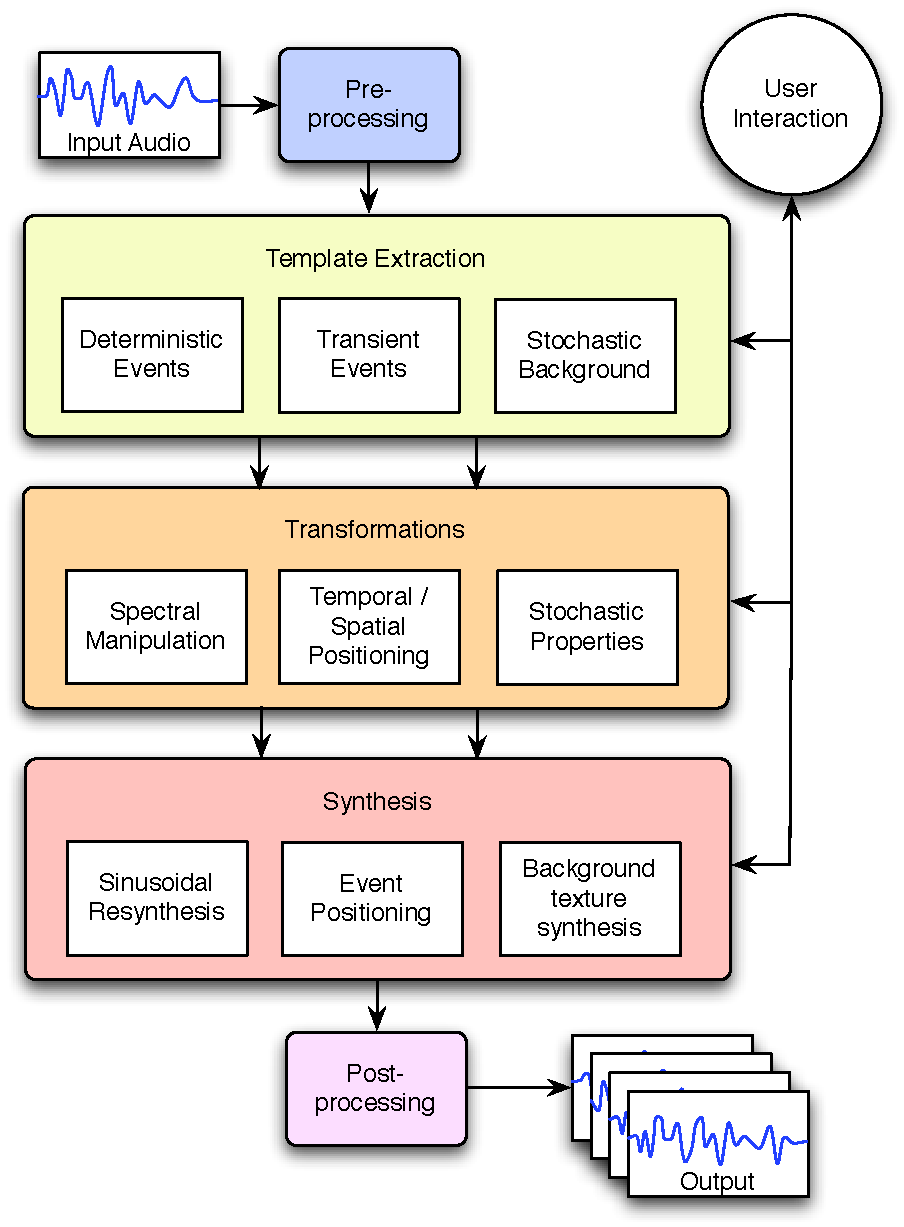
\includegraphics[width=\columnwidth]{pipeline.pdf} % was .9\columnwidth
\caption{TAPESTREA sound design pipeline.}
\label{fig:pipeline}
\end{figure}
TAPESTREA manipulates sound in several phases 
(see Figure~\ref{fig:pipeline}). 
In the analysis phase, desired parts of a recording are interactively extracted into templates of different types. Pitched components are saved as \textit{sinusoidal} templates~\cite{Serra89}. Brief noisy events are captured as \textit{transient} templates, using onset detection methods~\cite{Bello05}. The \textit{background} din is extracted by removing sinusoidal components in the frequency domain~\cite{Serra89} and replacing transient segments in the time domain. Each template can then be transformed independently, including structural changes to sinusoidal templates~\cite{Lieber08}. Time and frequency transformations are available for sinusoidal and transient templates, while background din may be continuously generated via wavelet tree learning~\cite{Dubnov02}. In the synthesis phase, these transformed templates can be combined using special \textit{synthesis} templates to produce a new composite soundscape or composition. A set of graphical user interfaces offers interactive parametric control over each phase of analysis, transformation and re-synthesis. ChucK scripting provides additional control over the synthesis through the simultaneous, precise manipulation of many parameters, and also provides an interface for input from external devices or user-defined GUI elements. 
%Description\\
%Main features

The TAPESTREA software is open-source, cross-platform, and freely available at \texttt{http://taps.cs.princeton.edu/}. A package containing the source code, license, documentation, and multimedia examples and demo can be downloaded at
\texttt{http://taps.cs.princeton.edu/tapestrea-acmm09.tgz}.\\
User support includes online documentation, a wiki, and a mailing list with 178 members. Web logs indicate that the software has been downloaded approximately 10300 times since April 2008; this statistic counts downloads of only the latest released version at any time, but does not account for bots or repeated downloads by the same person.

\section{Applications}

%Intended audience\\
%Applications
%Link to examples
%\subsection{Public usage information}
%Download statistics\\
%Histogram of how people use it
While TAPESTREA intends to aid sound design and composition from existing sounds, its applications include:
\begin{itemize}
\setlength\itemsep{-3pt}
\item Analysis, information extraction: Parametrically extracting a part of a recording, possibly gaining a better understanding of the sound through the analysis techniques and parameters that best capture it,
\item Synthesis, sound design, composition: Creating sound scenes for entertainment (such as games or video), and musical compositions (such as musique concr\`ete),
\item Pedagogy: Enhancing understanding of digital audio, signal processing, and computer music concepts via the interactive analysis, synthesis, and audiovisual display.
\end{itemize}

\begin{figure}[h]
\centering
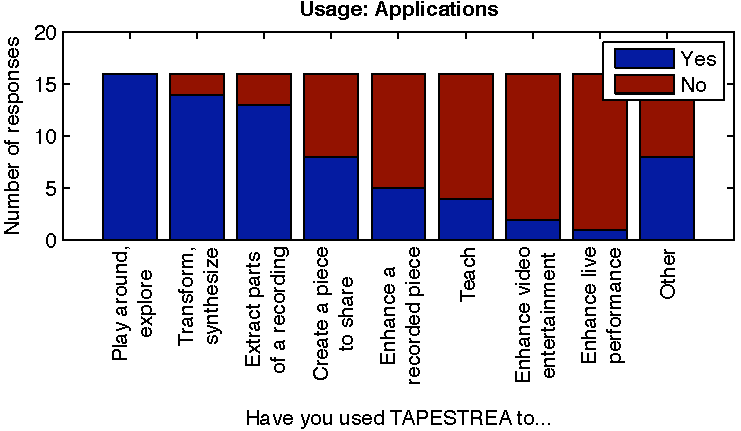
\includegraphics[width=\columnwidth]{usage_applications.pdf} %was .9\columnwidth
\caption{Applications for TAPESTREA usage.}
\label{fig:usage_applications}
\end{figure}

An informal survey of users on the TAPESTREA mailing list collected usage information. Voluntary responses to a series of yes/no questions are summarized in Figure~\ref{fig:usage_applications}. These provide an idea of how TAPESTREA has actually been used. All respondents reported having used it to ``play around and explore,'' while the majority of users also reported having used it to extract sound parts and to transform and synthesize templates. Half the users have used it to ``create a piece that [they] shared with others.'' A few have also used it for more specific arenas such as enhancing a recorded piece, teaching, enhancing video entertainment (like games or animations) and live performance. 

\section{Conclusions and Future Work}

TAPESTREA provides a new way to design sound through highly flexible manipulation of existing recordings. The tools and interface together provide great freedom in selecting which parts of a sound to re-use and how to transform and combine selected elements. The interactive coupling of analysis and synthesis techniques and paradigms make TAPESTREA stronger than the sum of its parts, leading to a comprehensive framework for manipulating existing audio. Thus, TAPESTREA presents a powerful tool for sound design, composition and pedagogy. Areas for further work include continuing to integrate user feedback to improve the software, as well as expanding it to provide even more powerful scripting, intelligent parameter suggestions via machine learning, and a meaningfully searchable database of extracted templates.

%ACKNOWLEDGMENTS are optional
%\section{Acknowledgments}
%This section is optional; it is a location for you
%to acknowledge grants, funding, editing assistance and
%what have you.  In the present case, for example, the
%authors would like to thank Gerald Murray of ACM for
%his help in codifying this \textit{Author's Guide}
%and the \textbf{.cls} and \textbf{.tex} files that it describes.

%
% The following two commands are all you need in the
% initial runs of your .tex file to
% produce the bibliography for the citations in your paper.
\bibliographystyle{abbrv}
\bibliography{fullnames,taps_acmm09}  % sigproc.bib is the name of the Bibliography in this case
% You must have a proper ".bib" file
%  and remember to run:
% latex bibtex latex latex
% to resolve all references
%
% ACM needs 'a single self-contained file'!
%
%APPENDICES are optional
%\balancecolumns
%\appendix
%%Appendix A
%\section{Headings in Appendices}
%The rules about hierarchical headings discussed above for
%the body of the article are different in the appendices.
%In the \textbf{appendix} environment, the command
%\textbf{section} is used to
%indicate the start of each Appendix, with alphabetic order
%designation (i.e. the first is A, the second B, etc.) and
%a title (if you include one).  So, if you need
%hierarchical structure
%\textit{within} an Appendix, start with \textbf{subsection} as the
%highest level. Here is an outline of the body of this
%document in Appendix-appropriate form:
%\subsection{Introduction}
%\subsection{The Body of the Paper}
%\subsubsection{Type Changes and  Special Characters}
%\subsubsection{Math Equations}
%\paragraph{Inline (In-text) Equations}
%\paragraph{Display Equations}
%\subsubsection{Citations}
%\subsubsection{Tables}
%\subsubsection{Figures}
%\subsubsection{Theorem-like Constructs}
%\subsubsection*{A Caveat for the \TeX\ Expert}
%\subsection{Conclusions}
%\subsection{Acknowledgments}
%\subsection{Additional Authors}
%This section is inserted by \LaTeX; you do not insert it.
%You just add the names and information in the
%\texttt{{\char'134}additionalauthors} command at the start
%of the document.
%\subsection{References}
%Generated by bibtex from your ~.bib file.  Run latex,
%then bibtex, then latex twice (to resolve references)
%to create the ~.bbl file.  Insert that ~.bbl file into
%the .tex source file and comment out
%the command \texttt{{\char'134}thebibliography}.
%% This next section command marks the start of
%% Appendix B, and does not continue the present hierarchy
%\section{More Help for the Hardy}
%The sig-alternate.cls file itself is chock-full of succinct
%and helpful comments.  If you consider yourself a moderately
%experienced to expert user of \LaTeX, you may find reading
%it useful but please remember not to change it.
%%\balancecolumns % GM June 2007
%% That's all folks!
\end{document}
